\newcommand{\secondLanguage}{icelandic} 			% if a second language is used, add it here
\documentclass[draft, {\secondLanguage}, english]{volcanica-template} 
\nonstopmode									% can toggle to see compilation warnings
\newcommand{\ArticleType}{Report}			
% Please choose between Research article, Report, Review, or Methods. 
% Details about different article types are available at: 
% https://www.jvolcanica.org/ojs/index.php/volcanica/about/submissions

%------------------------------------------------------------
%  Article details go here 
%------------------------------------------------------------	
\newcommand{\Title}{The Ethics of Artificial Intelligence for the Sustainable Development Goals} 	% Manuscript title goes here.
\newcommand{\shortTitle}{AI for SDGs} 		        % Short title for header goes here, less than 60 characters.
\newcommand{\Author}{P.Tahan A.Maci\xspace}    	% First author goes here.

%------------------------------------------------------------
%  Author details go here 
%------------------------------------------------------------	
\author[{{\affiliation{1}}}] 				% affiliation number
{\orcidaffil{0000.0000.0000.0000}~			% orcid number
Paria Tahan	 				% first author
\Email{paria.tahan@studenti.unipd.it}} 		        	% corresponding author email
\author[{{\affiliation{2}}}] 				% affiliation number
{\orcidaffil{0000.0000.0000.0000}~			% orcid number
Andrea Maci 			
\Email{andrea.maci@studenti.unipd.it}} 		% second author

%------------------------------------------------------------
%  Affiliations 		
%------------------------------------------------------------	
\affil[{{\affiliation{1}}}]{					% affiliation #1
2043889 paria.tahan@studenti.unipd.it; Department of Computer Engineering.
}
\affil[{{\affiliation{2}}}]{					% affiliation #2
2063146 andrea.maci@studenti.unipd.it; Department of Computer Engineering.
}

%------------------------------------------------------------
%  BIBLIOGRAPHY FILE 		
%------------------------------------------------------------	  
\addbibresource{bib-file.bib}		  		% add the name of the bibliography file here

%------------------------------------------------------------
%  Start of Document 		
%------------------------------------------------------------	  
\begin{document}

%------------------------------------------------------------
%  Abstract(s) and Keywords
%------------------------------------------------------------	
% Replace dummy text (\protect{\lipsum[45]}) with the abstract in the first argument for \FrontMatter (between the curly braces {}). 
% If there is a second-language abstract, it goes between the square brackets []. 
% Make sure you have included the correct language in line 1, above.
% If no second abstract, ensure there is no space between the square brackets [].
\FrontMatter{\protect{\lipsum[45]}}
[]% 
{					
\keywords{AI}{Climate change}{Agricultural management}{Rangeland monitoring}{Sustainable Development Goals}{Water}{Leak detection}{WSN}{Quality}{Monitoring}	% add up to six keywords in curly braces {}
}

%------------------------------------------------------------
%  Maintext
%------------------------------------------------------------	
\hypertarget{introduction}{%
\section{Introduction}\label{introduction}}		% Sections labelled and linked

Welcome to the \VOLCANICA research article \latex template. If you are already comfortable using \latex and \bibtex, you can go ahead and use the blank template (blank-template.tex). (If you're editing on Overleaf, you might want to change the "Main document" in Menu > Settings. You can also right-click to rename "blank-template" to something more relevant)

Otherwise, this template contains a bit more information to help you get started using \latex as a word processing software. Any issues or questions, email editor@jvolcanica.org.

Volcanica uses three levels of headings, which can be defined using "section", "subsection", and "subsubsection" commands.

\section{AI for Sustainable Agriculture and Rangeland Monitoring}\label{sec:02}
This paper \parencite{Efremova2023} explores the use of AI and satellite imagery in sustainable agriculture for resource allocation based on satellite monitoring results. A novel framework is proposed, incorporating AI and earth observation data, to address climate change-related challenges in the agri-food sector. The study identifies specific Sustainable Development Goals (SDGs) where AI can benefit practitioners, researchers, and policymakers. 

A case study involving a conservancy examines resource allocation decisions for optimal grazing and soil nutrition using cattle herds. Physical biomonitoring parameters are monitored through satellite imagery, and an AI-based approach is proposed for efficient interpretation. The results indicate that the framework enables real-time monitoring with accurate biomonitoring estimations and improved resource allocation practices aligned with SDG 2 \parencite{Efremova2023}.

\subsection{Problem Overview}\label{sec:02a}
We propose that the fundamental objective of the AI for SDGs framework is to accomplish SDG target 17.19, which entails establishing a structured partnership to develop alternative measures of progress in sustainable development that complement GDP. Currently, this target is primarily assessed by the monetary value of resources allocated to strengthen statistical capabilities in developing nations (SDG 17.19.1). AI for Good can contribute in three significant ways. Firstly, it can assist in reducing the costs associated with data collection and analysis. Secondly, it can help enhance measurement capabilities. This systematic approach ultimately enables more effective integration of AI solutions within direct interventions.

To progress in this direction, utilizing AI in conjunction with earth observation data (EO) is a crucial step. The combination of AI and EO offers a dependable and detailed dataset that enables improved monitoring of the Sustainable Development Goals (SDGs). The provided Table 1 outlines the primary functions of AI within an evaluative infrastructure, commencing with its role in mapping, which is reliant on earth observation data.


The authors argue that agriculture and rangeland management are facing increasing pressure to become more sustainable due to a growing global population, climate change, and other environmental challenges. In order to meet these challenges, there is a need for more efficient and effective monitoring of crops, livestock, and rangelands. However, traditional methods of monitoring can be time-consuming, expensive, and may not provide the level of detail needed to make informed decisions. This is where artificial intelligence (AI) can play a role by providing a means to analyze large amounts of data and identify patterns and trends that can be used to improve decision-making in agriculture and rangeland management.

However, the authors also acknowledge that there are challenges that need to be addressed for AI to be used in a way that benefits farmers, ranchers, and the environment. These challenges include the need for accurate and reliable data, the need for AI algorithms that are tailored to specific contexts and environments, and the need to address ethical and social issues related to the use of AI in agriculture and rangeland management. The authors argue that by addressing these challenges, AI has the potential to support sustainable agriculture and rangeland management and contribute to the achievement of the United Nations' Sustainable Development Goals.
\subsubsection{AI-EO SDG Model: Zero Hunger}\label{sec:02aa}
In this section, we provide a brief overview of the problem of hunger and malnutrition, which is the focus of the AI-EO SDG Model for Zero Hunger. The authors note that despite significant progress in reducing hunger and malnutrition in some parts of the world, many people still suffer from hunger and malnutrition, particularly in sub-Saharan Africa and South Asia. In addition, the COVID-19 pandemic has exacerbated food insecurity and disrupted food systems around the world.

The authors also highlight the complexity of the problem of hunger and malnutrition, which is influenced by a wide range of factors, including poverty, conflict, climate change, and inadequate access to education and health services. They argue that addressing this complex problem requires a multi-faceted approach that integrates a range of interventions, from increasing agricultural productivity and improving access to nutritious foods, to strengthening social safety nets and promoting gender equality. The AI-EO SDG Model aims to contribute to this multi-faceted approach by using artificial intelligence and Earth observation data to support evidence-based decision-making and monitoring of progress towards the goal of zero hunger.

\subsubsection{AI-EO SDG Model: Climate Change}\label{sec:02ab}
The other problem that should be covered in the AI-EO SDG model is climate change. It is notable that climate change is one of the most pressing challenges facing the world today, with its impacts already being felt in the form of more frequent and severe weather events, rising sea levels, and increased frequency and intensity of wildfires and droughts. These impacts have significant implications for a range of sectors, including agriculture, energy, transportation, and infrastructure, and are likely to exacerbate existing inequalities and vulnerabilities.

The complexity of the problem of climate change, which is caused by a range of human activities, including the burning of fossil fuels, deforestation, and industrial and agricultural practices should be highlighted. Addressing this complex problem requires a multi-faceted approach that involves reducing greenhouse gas emissions, building resilience to the impacts of climate change, and transitioning to a more sustainable and low-carbon economy. The AI-EO SDG Model aims to contribute to this approach by using artificial intelligence and Earth observation data to support decision-making and monitoring of progress towards the goal of mitigating and adapting to climate change.

\subsection{Background}\label{sec:02b}
\subsubsection{Rangelands}\label{sec:02ba}
In this section we will focus on the Rangelands which are natural landscapes that are used for grazing livestock and provide important ecosystem services, such as carbon storage, water regulation, and biodiversity conservation. The authors note that rangelands cover a significant portion of the Earth's land surface, with an estimated 25\% of the world's land area classified as rangelands. However, rangelands are under increasing pressure from a range of factors, including climate change, land use change, and overgrazing, which can lead to soil degradation, loss of biodiversity, and reduced capacity to sequester carbon.

The authors argue that addressing the challenges facing rangelands requires a multi-faceted approach that incorporates a range of interventions, from improving livestock management practices and reducing overgrazing to promoting sustainable land use practices and restoring degraded ecosystems. The AI-EO SDG Model aims to contribute to this approach by using artificial intelligence and Earth observation data to support decision-making and monitoring of progress towards the goal of sustainable management of rangelands. The authors provide examples of how the model can be used to estimate biomass production, monitor vegetation cover, and identify areas at risk of degradation, among other applications.
\subsubsection{AI for Climate Change and Agriculture: Overview}\label{sec:02bb}
In this section, we explain the use of AI in addressing the challenges of climate change and agriculture. The authors note that AI has the potential to support decision-making and enhance the efficiency and effectiveness of agricultural systems, by providing insights into weather patterns, crop growth, and soil health. AI can also be used to develop predictive models of climate change impacts, identify areas at risk of soil erosion and degradation, and improve the efficiency of irrigation systems.

The authors highlight several examples of AI applications in agriculture, including precision agriculture, which uses sensors and machine learning algorithms to optimize crop yields while reducing inputs such as water and fertilizer. They also discuss the use of AI in supporting climate-smart agriculture, which seeks to promote sustainable land use practices that reduce greenhouse gas emissions, enhance the resilience of agricultural systems to climate change, and increase the productivity and income of smallholder farmers. The AI-EO SDG Model aims to contribute to these efforts by integrating AI and Earth observation data to support evidence-based decision-making and monitoring of progress toward the goal of sustainable agriculture and climate change mitigation and adaptation.
\subsection{Methods}\label{sec:02c}
\subsubsection{Overview of the Proposed Approach}\label{sec:02ca}
This section provides an in-depth overview of the proposed approach of the AI-EO SDG Model for Climate Change. The authors note that the model will be designed to integrate artificial intelligence and Earth observation data to support decision-making and monitoring of progress toward the goal of climate change mitigation and adaptation. They explain that the approach will be based on a multi-faceted framework that incorporates a range of data sources, including satellite imagery, climate models, and socio-economic data, to provide a comprehensive understanding of the complex interactions between human and natural systems.

The authors highlight several key components of the proposed approach, including the development of machine learning algorithms to analyze large volumes of Earth observation data and generate actionable insights for decision-makers. They explain that these algorithms will be trained on historical data and will use a range of techniques, such as deep learning and neural networks, to identify patterns and trends in the data. The authors also note that the model will incorporate climate models to develop predictive models of climate change impacts, which can be used to inform decision-making and support climate adaptation strategies.

In addition, the authors emphasize the importance of incorporating socio-economic data into the model, in order to understand the human dimensions of climate change and support the development of climate-smart policies and interventions. They explain that this will involve integrating data on factors such as population density, land usepatterns, and economic activity, and using this information to identify vulnerable populations and areas at risk of climate change impacts. The authors note that the model will be designed to be flexible and scalable, allowing it to be adapted to different contexts and used by a range of stakeholders, from policymakers to farmers and other land managers. Overall, the proposed approach of the AI-EO SDG Model aims to provide decision-makers with a comprehensive and integrated understanding of the complex interactions between human and natural systems, in order to support evidence-based decision-making and monitoring of progress towards the goal of sustainable development.

\subsubsection{Data}\label{sec:02cb}
In this section, we discussed about the data sources used in the AI-EO SDG model. The authors note that the model will incorporate a wide range of data sources, including satellite imagery, climate models, and socio-economic data. They explain that these data sources will provide a comprehensive understanding of the complex interactions between human and natural systems that are critical to addressing the challenge of climate change.

The authors highlight the importance of Earth observation data in providing information on key environmental indicators, such as land cover, vegetation indices, and soil moisture. They note that this data can be used to monitor changes in the environment, identify areas at risk of degradation, and support the development of climate-smart land use policies. The authors also emphasize the importance of climate models in developing predictive models of climate change impacts, which can be used to inform decision-making and support climate adaptation strategies. Finally, the authors note that the model will incorporate socio-economic data to understand the human dimensions of climate change and support the development of climate-smart policies and interventions.

\subsubsection{Model Architecture}\label{sec:02cc}

\begin{figure*}[!t]								%[tbhp]
\centering
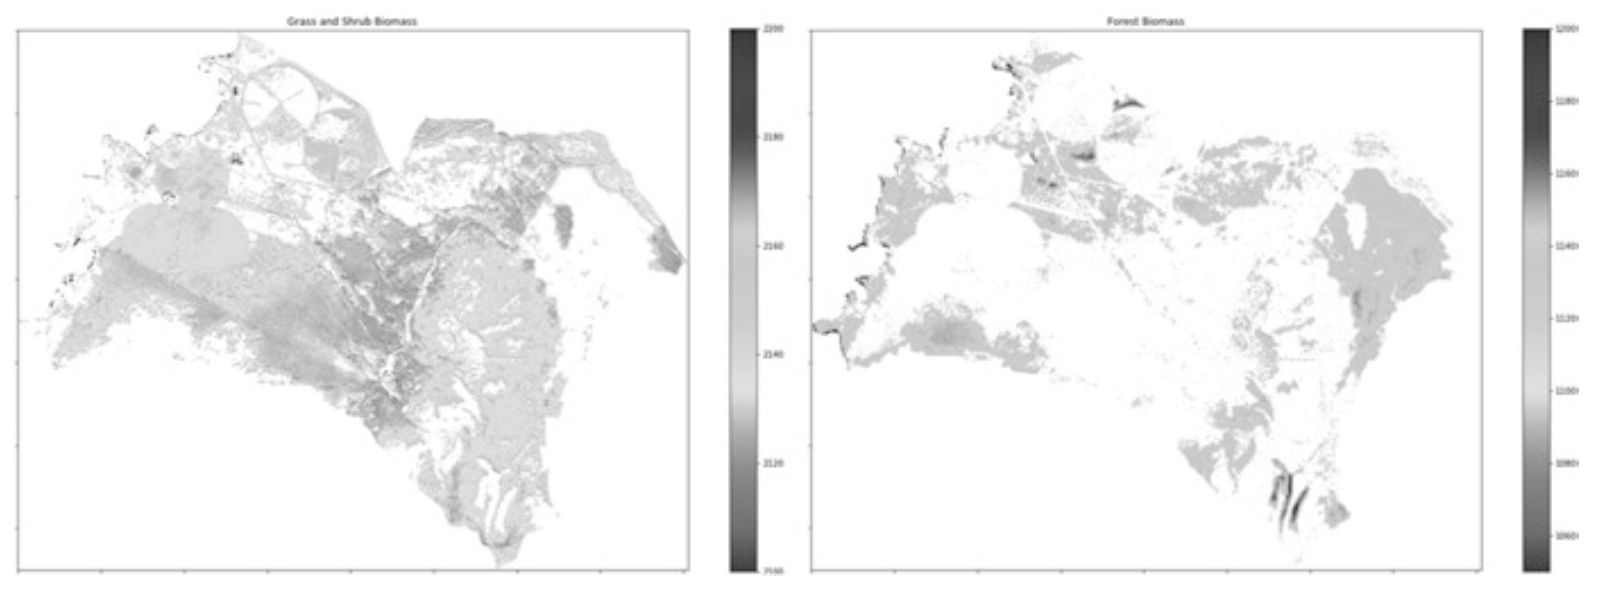
\includegraphics[width=\textwidth]{Images/fig1-3.png}
\caption{Biomass estimation for grassland, shrublands, and forest land cover types}	
\label{fig:01}									
\end{figure*}

The authors note that the model will be designed to integrate artificial intelligence and Earth observation data to support decision-making and monitoring of progress toward the goal of climate change mitigation and adaptation. They explain that the model will be based on a modular architecture that allows for flexibility and scalability and will be designed to integrate a range of data sources, including satellite imagery, climate models, and socio-economic data.

The authors describe the three main modules that will make up the model architecture: the data processing module, the feature extraction module, and the predictive modeling module. The data processing module will be responsible for pre-processing and cleaning the data, and will include functions for ingesting data from a range of sources, such as satellite sensors, climate models, and socio-economic databases. The module will also include tools for data quality control, data normalization, and data transformation, in order to ensure that the data is accurate, reliable, and consistent. The feature extraction module will be responsible for identifying relevant features and patterns in the data, using a range of techniques such as machine learning algorithms and statistical analyses. The module will also include tools for feature selection, feature engineering, and dimensionality reduction, in order to reduce the complexity ofthe data and improve the efficiency of the predictive modeling module.

The predictive modeling module will be responsible for developing machine learning algorithms that can generate actionable insights from the data. The authors explain that the module will use a range of techniques, such as deep learning, neural networks, and decision trees, to generate models that can predict key outcomes related to climate change, such as changes in temperature, precipitation, or vegetation cover. The module will also incorporate uncertainty and sensitivity analyses, in order to provide decision-makers with a range of possible scenarios and their associated risks and opportunities.

The authors also describe several important sub-modules that will be integrated into the model architecture. These include the data integration and fusion sub-module, which will be responsible for integrating and fusing data from different sources, in order to provide a comprehensive and integrated understanding of the complex interactions between human and natural systems. The sub-module will include tools for data mapping, data harmonization, and data fusion, in order to ensure that the data is consistent and standardized across different sources.

Another important sub-module is the feedback and evaluation sub-module, which will be responsible for evaluating the performance of the model and incorporating user feedback into the model development process. The sub-module will include tools for model validation, model comparison, and model improvement, in order to ensure that the model is accurate, reliable, and relevant to the needs of decision-makers.

Overall, the modular architecture of the AI-EO SDG Model for Climate Change aims to provide a flexible and scalable framework for integrating artificial intelligence and Earth observation data to support decision-making and monitoring of progress toward the goal of climate change mitigation and adaptation. The authors note that the modular approach will allow for the integration of new data sources and modules as they become available, and will enable the model to be adapted to different contexts and used by a range of stakeholders, from policymakers to farmers and other land managers.

\begin{figure*}[!t]								%[tbhp]
\centering
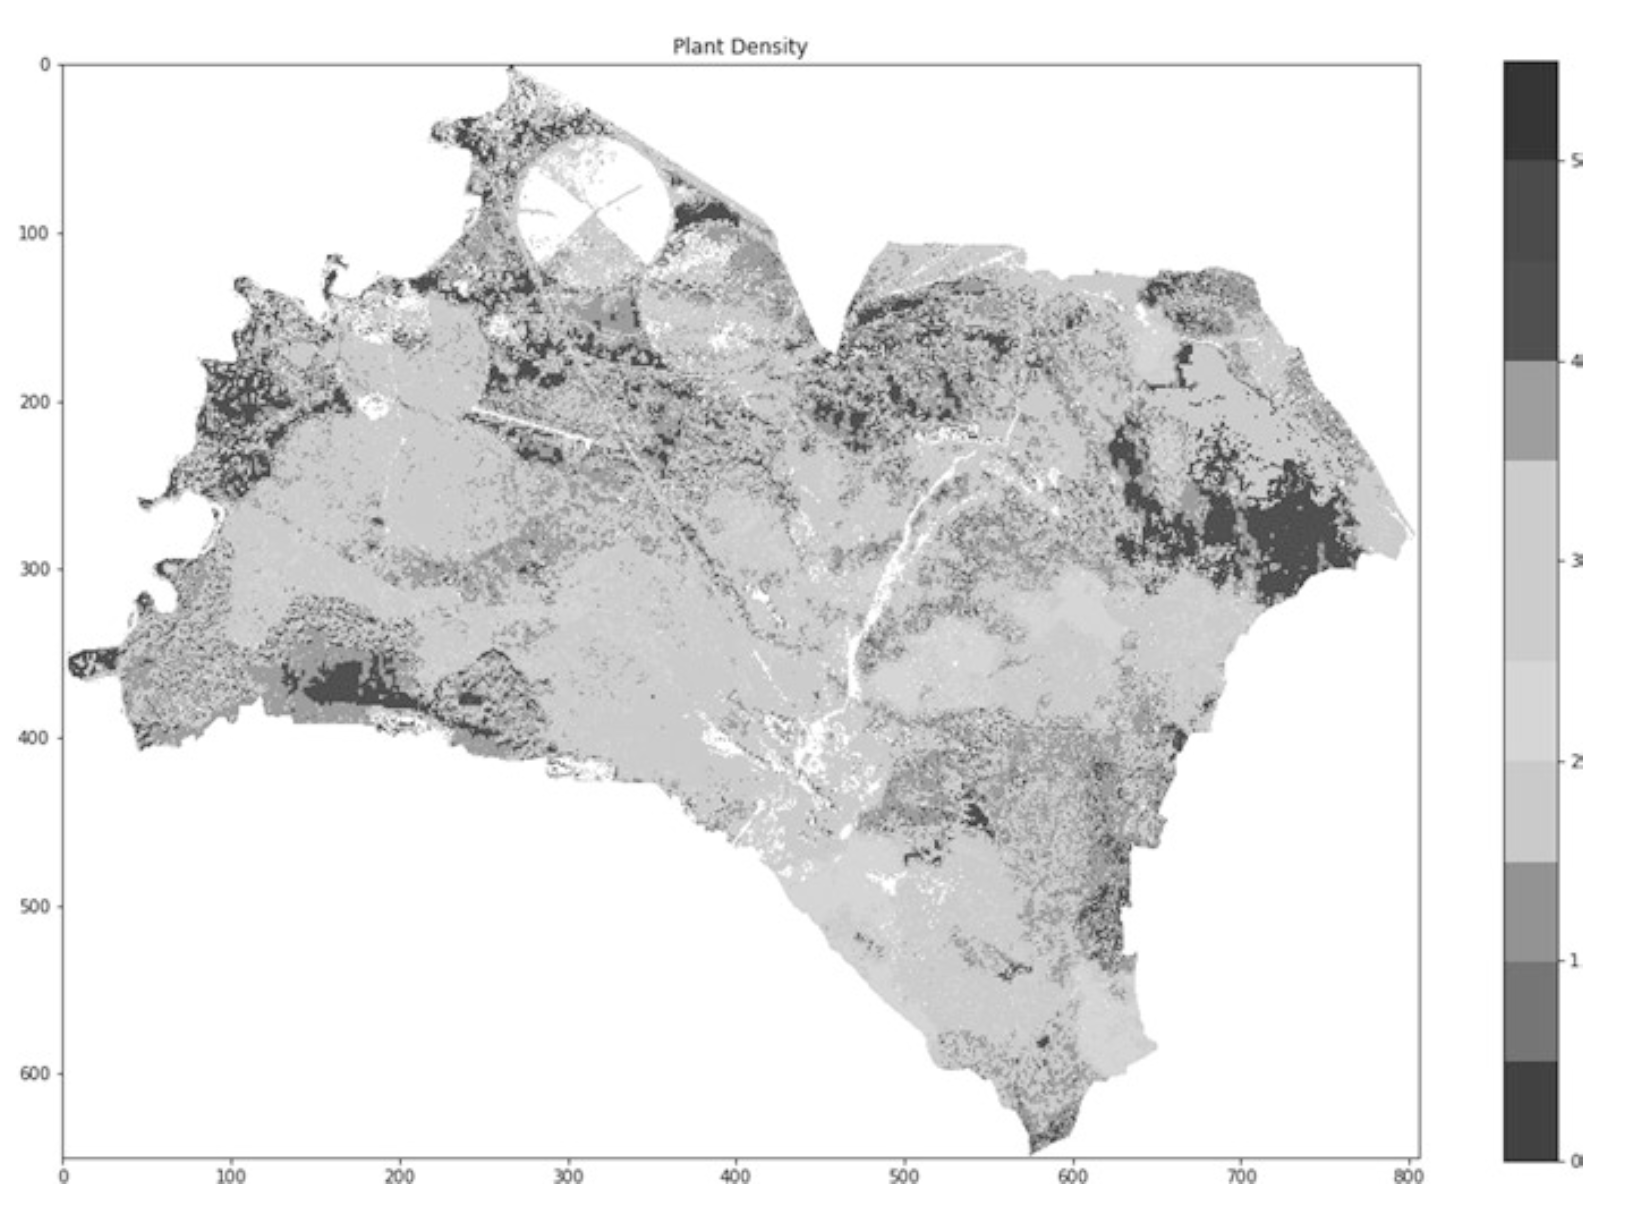
\includegraphics[width=\textwidth]{Images/fig2-3.png} 
\caption{Estimation of plant density across the rangelands. The colour coding shows the highest vegetation areas as blue and the lowest as red, respectively
}	
\label{fig:02}									
\end{figure*}

In addition to the three main modules, the authors also describe several other important sub-modules that will be integrated into the model architecture. These include the sensor calibration and validation sub-module, which will be responsible for ensuring the accuracy and reliability of the satellite sensors used to collect Earth observation data. The sub-module will include tools for sensor calibration, sensor validation, and data quality control, in order to ensure that the data is accurate and reliable.

Another important sub-module is the data visualization and communication sub-module, which will be responsible for presenting the data and the insights generated by the model in a clear and understandable way. The sub-module will include tools for data visualization, data exploration, and data communication, in order to enable decision-makers to understand the implications of the data and the insights generated by the model.

\begin{figure*}[!t]								%[tbhp]
\centering
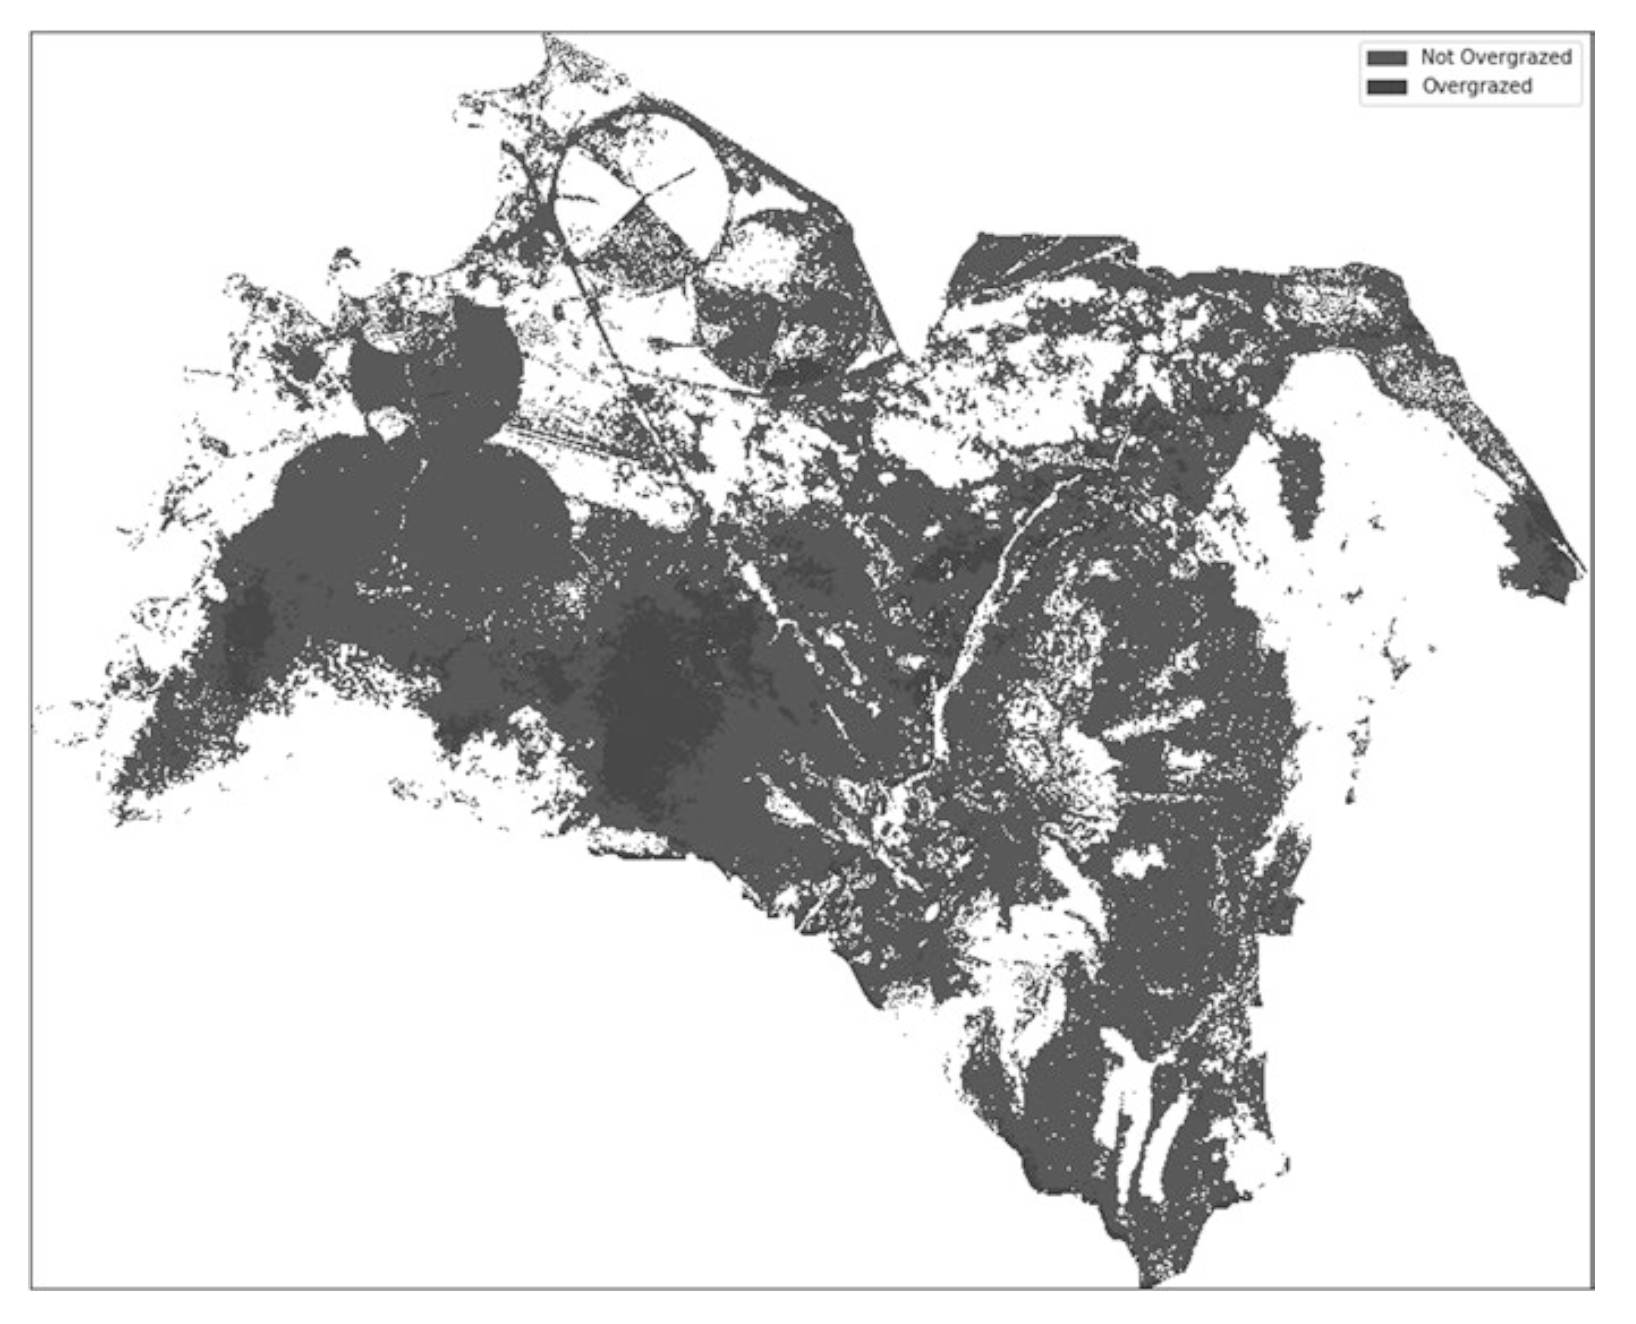
\includegraphics[width=\textwidth]{Images/fig3-3.png} 
\caption{Overgrazing prediction. Red areas indicate the places with the highest degrees of overgrazing}	
\label{fig:03}									
\end{figure*}

Finally, the authors note that the model architecture will incorporate a cloud-based infrastructure, which will enable the model to be easily accessed and used by a wide range of stakeholders. The infrastructure will include tools for data storage, data sharing, and data analysis, and will be designed to be scalable and secure, in order to ensure the privacy and security of the data. The authors emphasize that the cloud-based infrastructure will enable the model to be easily scaled up or down, depending on the needs of users, and will enable the model to be accessed from anywhere in the world, using a range of devices.

Overall, the authors argue that the modular architecture of the AI-EO SDG Model for Climate Change provides a flexible and scalable framework that can be adapted to different contexts and used by a range of stakeholders. The authors emphasize that the model will be designed to be user-friendly and accessible, even for those with limited technical expertise, in order to enable decision-makers at all levels to make informed decisions and monitor progress toward the goal of climate change mitigation and adaptation. The authors conclude that the AI-EO SDG Model for Climate Change has the potential to make a significant contribution to the global effort to address the challenge of climate change, by providing decision-makers with a comprehensive and integrated understanding of the complex interactions between human and natural systems.

\subsection{Discussion}
The model has the potential to support evidence-based decision-making and monitoring of progress towards the goal of climate change mitigation and adaptation. They argue that the model can provide decision-makers with a comprehensive and integrated understanding of the complex interactions between human and natural systems, and can support the development of climate-smart policies and interventions. The authors also note that the model can provide critical information to smallholder farmers and other land managers, enabling them to make informed decisions about land use and crop management.

The authors conclude that the Model has the potential to make a significant contribution to the global effort to address the challenge of climate change, and can support the achievement of the Sustainable Development Goals related to climate change and sustainable agriculture.

\begin{figure*}[!t]								%[tbhp]
\centering
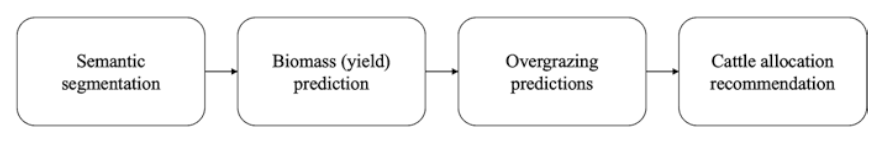
\includegraphics[width=\textwidth]{Images/fig4-3.png} 
\caption{Model implementation for efficient resource allocation}	
\label{fig:04}									
\end{figure*}

\subsubsection{Challenges and Economic Implications}
The authors note that one of the main challenges will be the availability and accessibility of data, particularly in developing countries, where data infrastructure may be limited. They also highlight the need for capacity building and technical training to enable decision-makers to effectively use the model and interpret the insights it generates. In terms of economic implications, the authors note that the model has the potential to generate significant economic benefits, particularly in the agricultural sector, by enabling farmers to make more informed decisions and improve their yields. However, the authors also caution that the model may have implementation costs, particularly related to data processing and storage, and note that these costs will need to be carefully considered when planning for the implementation of the model.

\subsubsection{Economic Outcomes}
The authors note that the model has the potential to generate significant economic benefits, particularly in the agricultural sector, by enabling farmers to make more informed decisions and improve their yields. The authors also highlight the potential for the model to support the development of new climate-smart technologies and services, such as improved weather forecasting and water management systems, which can create new business opportunities and drive economic growth. However, the authors caution that the model may also have implementation costs, particularly related to data processing and storage, and note that these costs will need to be carefully considered when planning for the implementation of the model. Overall, the authors argue that the economic benefits of the AI-EO SDG Model for Climate Change are significant and have the potential to contribute to sustainable development and poverty reduction goals.

\autoref{sec:02} or \autoref{sec:02a}. The autoref command can also be used to refer to figures, tables, and other items. Here's an example of how to include a single-column-width figure:

%------------------------------------------------------------
%  Single column figure
%------------------------------------------------------------	
\begin{figure}[!b]								%[tbhp]
\centering
\includegraphics[width=\columnwidth]{example-image} % inside { } should be the path to the image file
\caption{This is where a descriptive caption goes. A good idea is to include all your figures in a specific folder (e.g. "media") within the Overleaf project (or the same directory as the .tex file, if you are editing offline). The path to the figures then looks like "media/figure-1.pdf". PDF, SVG, or other vector graphics are preferred formats, but high-resolution image formats (e.g. PNG or JPG) are also acceptable.}		% Include the figure caption here
\label{fig:011}			% Include a unique label here, so you can refer to the figure
\end{figure}
%------------------------------------------------------------	

Figure references look like this: \autoref{fig:01}. Sometimes you might want to include a wider figure; the command for this looks slightly different:
%------------------------------------------------------------
%  Double column figure
%------------------------------------------------------------	
\begin{figure*}[!t]								%[tbhp]
\centering
\includegraphics[width=\textwidth]{example-image-a} % inside { } should be the path to the image file
\caption{This is where a descriptive caption goes.}	% Include the figure caption here
\label{fig:022}									% Include a unique label here, so you can refer to the figure
\end{figure*}
%------------------------------------------------------------	

If you want to use mathematical symbols and short in-line equations, just wrap them in dollar signs: $mx +c$. Larger equations go in their own kind of special environment called, unsurprisingly, equation.
%------------------------------------------------------------
%  Equation
%------------------------------------------------------------	
\begin{equation}
S(\omega) = \frac{\alpha g^2}{\omega^5} \exp\Bigl[ -0.74\Bigl\{\frac{\omega U_\omega 19.5}{g}\Bigr\}^{\!-4}\,\Bigr] 
\label{eq:01}\end{equation}
%------------------------------------------------------------	
These can also be labelled and referred to (see \autoref{eq:01} above). Subequations can also be typeset, as shown in \autoref{eq:02} below.

%------------------------------------------------------------
%  Sub-equations
%------------------------------------------------------------	
\begin{subequations}
\begin{align}
v_x &= v_0 \cos(\theta)\exp\bigg(-\frac{g}{v_t}t\bigg) \label{eq:2a}\\[0.5ex]
v_y &=v_0\sin(\theta)\exp\bigg(-\frac{g}{v_t}t\bigg)-v_t\bigg[1-\exp\bigg(-\frac{g}{v_t}t\bigg)\bigg]. \label{eq:2b}\end{align}
\label{eq:02}
\end{subequations}
%------------------------------------------------------------

\section{Smart Control of Drinking Water Grids Using IoT}
In the second paper [INSERT REFERENCE], the authors discuss the application of Internet of Things (IoT) technology in the smart control of drinking water grids. The authors begin by discussing the importance of water, particularly in relation to human life and the challenges associated with maintaining its quality. Water is in fact a vital chemical component for life and its significance continues to increase with the needs of modern civilization. However, the quality of distributed drinking water has become a crucial factor affecting public health and economic development in many parts of the world. Poor water supply and sanitation conditions, especially in developing countries, contributes to approximately 80\% of the total diseases. The article highlights how IoT can revolutionize the management and monitoring of water distribution systems by providing real-time data and enabling efficient control and optimization of operations, as opposed to traditional slow and inefficient methods.

\subsection{Problem Overview}
The conventional methods of monitoring water quality involve manual collection of samples, which are then tested in laboratories. However, this approach is deemed inefficient, expensive, time-consuming, and lacks real-time results. To address this, the paper suggests the use of wireless sensor networks (WSNs) for continuous monitoring of drinking water quality. WSNs are self-configuring networks consisting of small sensor nodes that communicate with each other through radio signals. They are deployed to monitor physical or environmental conditions and transmit data to a central location for analysis. However, WSNs face challenges such as resource constraints, unreliable communication links, and low data rates. As a result, new protocols and algorithms have been developed specifically for WSN environments. The purpose of the work is to create an intelligent system for monitoring the quality of distributed drinking water, using a WSN to detect real-time contamination in the water distribution network and to address the issue of leaks in water pipes.

\subsubsection{Related works}
Before diving into the proposed architecture, the authors mention the importance of previous works in the literature, splitting them in two categories: those who focus on the monitoring of drinking water quality and those who focus on controlling leaks in water pipes.

\subsubsection{Water Quality Monitoring Systems}
Several systems for monitoring water quality have been developed. One possible system requires to measure the quality based on pH, water turbidity and temperature sensors; this is a practical and economical solution to monitor the water quality, especially in rural areas.
Another system instead exploits an IoT-based solution. This system provides remote monitoring of water quality along with water fow control via mobile application. The system classifies water quality using machine learning algorithms such as support vector machines (SVM) and deep learning neural networks.
A WSN based solution proposes to gather data about the water through pH, oxygen density and turbidity sensors. The sensors are powered by a solar power module, while the node to base station communication is realized via WSN technology.

\subsubsection{Leak Detection Solutions in the Water Distribution Network}
There are two main systems to detect leaks in water pipes. A static detection system relies on sensors and data collectors that are placed in the water distribution network. This data is periodically sent to the network management center to discover possible leaks. A dynamic detection system relies on the mobility of leak detection devices to an area where there is a suspected leak to conduct an investigation. The first system is prone to false alarms, while the latter immediately locates a leak under the assumption of already knowing the possibility of a leak. Acoustic technologies are the most commonly used in these systems. Other possible techniques involve time domain refectometry (TDR), ground-penetrating radar (GPR), and electrical resistivity tomography (ERT), experimented in underground pipes. Novel techniques utilizing machine learning and advanced statistical methods have been recently developed for the detection and approximate location of leaks.

\subsection{The Proposed System Architecture}
The proposed architecture develops a real-time system that monitors the water quality according to physicochemical and microbiological parameters, plus the system uses a data aggregation algorithm to improve the performance of the classification algorithms. The architecture also makes use of a control system for small and large leaks simultaneously, because those leaks belong to different categories and previous systems in the literature did not make this distinction.
\subsubsection{Architecture Overview}
The system consists of a computer platform and a wireless sensor network (WSN) that covers the water distribution network. The WSN is composed of sensor nodes and base stations, with each base station communicating with the control center through a computing platform. The platform includes modules for data collection, data visualization for operators to detect possible malfunctions thanks to sensors, data management to assess the validity of the current data, and long-term storage for in-depth database analyses.
The platform has specific requirements for industrialization, such as scalability to handle increasing amounts of data, flexibility for integration with other applications, and real time process management to ensure that the platform executes all modules in real time. To monitor the physicochemical quality of drinking water, the system adopts a WSN architecture with libelium smart water sensors. These sensors collect parameters such as pH, temperature, turbidity, and conductivity, and the data is routed to the sink nodes through Zigbee links. A Zigbee link is a low-power wireless mesh network standard in battery-powered devices in wireless control and monitoring applications, granting low latency communication. The sink nodes transmit the data to the control center using 4G radio links. For monitoring microbiological parameters, flow cytometers called bactosense are installed in water tanks and pumping stations. These sensors detect microbial cell numbers in the water by measuring parameters like live dead count and total cell count. The collected data from both physicochemical and microbiological sensors is transmitted to the control center.
\subsubsection{Leak Detection}
Since most pipes are installed underground, the authors propose to install, at each pipe junction, a pair of sensors. One sensor measures the water pressure in the pipe, useful to detect large leaks. The other sensor detects the nearby soil moisture, designed to locate small leaks, since these leaks don't affect the water pressure inside the pipe. Communication between network nodes is through Bluetooth links, and the data is transmitted from node to node until it reaches a base station in a pumping station or water treatment center. The base stations use 4G radio links to transmit the data to the control center.
\subsection{A New Model for Water Quality Analysis Based on Machine Learning}
The proposed model is based on three phases: data gathering from different sources, data aggregation, and classification using machine learning techniques.
\subsubsection{Data Gathering and Aggregation}
In order to test and experiment with the system, the authors chose to use the database of the water station “Ghadir El Golla” of Tunis-Tunisia. The database consists of 38 physicochemical and microbiological water quality parameters and 103 records for the year 2018. The data includes real measurements with respective standard errors.
As far as the data aggregation is concerned, the system is made up of $n$ sensors that gathers data for $p$ parameters. The data is gathered with interval $\Delta_k$, and, at each new interval, there are$m$ measurements per sensor.

%------------------------------------------------------------
  %SIMPLE TABLE
%------------------------------------------------------------	
\begin{table}[!thbp]
\centering
\caption{Caption goes up here.}
\begin{tabular}{
S[table-format=3.1]								% S-type column aligns decimals
S[table-format=3.3]								% x.y = #digits before and after decimal
S[table-format=2.2]
}
\toprule										% toprule
{Parameter 1} & {Parameter 2} & {Parameter 3} \\	% text in an S-type column must be enclosed in { }
\midrule										% midrule
3.8 	& 0.003	& 15.91	\\
1.4 	& 0.001	& 12.12	\\
21 	& 0.018	& 81.43	\\
0.8 	& 0.004	& 1.8		\\ [5pt]					% additional space every four lines
4.0 	& 0.004	& 14.76	\\
2.1 	& 0.003	& 13.31	\\
3.7 	& 0.006	& 16.48	\\
119 	& 0.02	& 83.01	\\ [5pt]
3.0 	& 0.001	& 15.2	\\
2.9 	& 0.002	& 11.01	\\

\bottomrule									% bottomrule
\end{tabular}
\label{tab:01}
\end{table}
%------------------------------------------------------------

Tables can become quite complex. A great resource is \url{https://www.tablesgenerator.com/latex_tables}, where you can paste table data, or load in an excel file, then copy the LaTeX output. Note that for two-column tables, the "table*" environment should be used, rather than the unstarred "table" environment.

\section{Citations}
To cite other articles, you need a .bib file. This is a separate file (in the same folder as the .tex and .cls files) which contains all the necessary bibliographic information. Two good resources compiling a .bib file are \url{https://www.doi2bib.org/} and \url{https://scipython.com/apps/doi2bib/}. Both of these allow you to enter an article's DOI number and retrieve the bibtex entry (which you can copy/paste into the .bib file). Bibtex entries can also be obtained via Google Scholar, by clicking "cite" > "bibtex". However, GS \emph{doesn't} include DOI numbers, so you may want to add these manually. Many reference managers (e.g. Zotero) allow authors to export a .bib file. Once you have a .bib file, citations are simple, both in-line, such as \textcite{Farquharson2018}, or in parentheses \parencite{Kavanagh2022}. The reference list will be formatted and printed automatically. Note that you can refer to multiple citations at once \parencite[e.g.][among others]{Kavanagh2022, Siebert2015}.

\section{Useful commands}

If you are using a lot of isotopes or isotopic ratios, you can use the commands "iso" and "isorat", which give outputs like \iso{C}{14} and \isorat{O}{18}{16}. Chemistry can be typeset using the "ch" command, giving output like \ch{H2SO4} or \ch{[AgCl2]-}, or even \ch{KCr(SO4)2 * 12 H2O}. There is also an "okina" command, as in Hawai{\okina}i. Here are some Greek letters: $\alpha$, $\beta$, $\phi$, $\Omega$. If we use software, like \software{Eject!}, it will look like this, using the command "software" or its alias "sw". Same goes for \sw{DensityX}, \sw{ImageJ}, and \sw{VolCalc}. SI units can be typeset using the "SI" command (SI{value}{unit}), where  unit is typed out: \SI{2600}{\kilo\gram\per\meter\cubed}. If there are symbols or commands you'd like to see incorporated in our templates, please reach out to farquharson@jvolcanica.org.

\Contributions{Who did what?% Author Contribution statement
}
%
\Acknowledgments{Any pertinent acknowledgements. Where applicable, funding sources should be provided here.% Acknowledgements statement.
}
%
\DataAvailability{Links to data repositories, and/or a statement regarding the availability of data here. Authors are encouraged to make data freely available wherever possible: we recommend free repositories such as Zenodo and FigShare in order to facilitate transparent open access. We recommend  versioning, archiving, and sharing code via GitHub/Zenodo; see: https://docs.github.com/en/repositories/archiving-a-github-repository/referencing-and-citing-content.% Data Availability statement
}
%
\EndMatter
\end{document}